\documentclass{template/acm_proc_article-sp}

\usepackage{graphicx}
\usepackage[utf8]{inputenc}
\usepackage[english]{babel}
\usepackage{hyperref}
\usepackage{listings}
\usepackage{siunitx}
\usepackage{csvsimple}
\usepackage{subcaption}
\usepackage{amsmath}

\begin{document} 

\title{Image tamper detection based on demosaicing artifacts}

\numberofauthors{2} 
\author{
% 1st. author 
\alignauthor
Matjaž Mav\\
       \affaddr{Faculty of Computer and Information Science, University of Ljubljana}\\
       \email{mm3058@student.uni-lj.si}
% 2nd. author
\alignauthor
Klemen Jesenovec\\
       \affaddr{Faculty of Computer and Information Science, University of Ljubljana}\\
       \email{kj9807@student.uni-lj.si}
}

\maketitle
\begin{abstract}
TODO
\end{abstract}

\keywords{TO, DO}

\section{Introduction}
This paper aims to review and summarize a paper about image tamper 
detection in the field of digital image forensics~\cite{dirik2009image}.

The paper classifies image tampering into three groups: 
\begin{description}
    \item[Targeted Tamper Detection] Which focus on detecting specific groups of 
    tampering such as re-compression, cloning, resizing, etc. 
    \item[Universal Tamper Detection] Which can only determine if the image
    was tampered with or not.
    \item[Localized Tamper Detection] Which can identify parts of the image 
    that were tampered with.
\end{description}

The paper describes a Color Filter Array (CFA) demosaicing based tamper detection
that can detect both local and global tempering.
The method works due to the fact that image tampering usually alters CFA demosaicing
artifacts in a way that can be detected and can thus detect a wide range of tampering
techniques. 

In the following chapters we explain CFA, summarize the technique presented 
in the original paper and present our own implementation in MATLAB.
Finally, we discuss the results and limitations of our implementation and compare it
to the results in the original paper.

\section{Color filter array}
Color filter array is a grid of small color filters put over an image sensor.
The filters are needed due to the sensor's inability to capture wavelength 
information and thus cannot distinguish between different colors.
The CFA filters out specifi
This enables cameras to capture color information.

\begin{figure}
\centering
\includegraphics[trim=175 200 100 205,clip,width=0.46\textwidth]{report/results/4_bayer_filters.jpg}
\caption{Commonly used Bayer filters}
\label{img_4_bayer_filters}
\end{figure}

\section{CFA Interpolation}
Bayer filter and different interpolation techniques, other filters X3...

\section{Image tampering categories}

\section{Review of other methods}


\section{CFA based features}
In this section we will review two CFA based features introduced in the paper \cite{dirik2009image}. The first feature (we will call it F1) mainly relies on the estimation of the source digital camera CFA pattern. And the second feature (we will call it F2) relies on the source digital camera sensor noise.

For both of the features we implemented algorithm in MATLAB. First evaluated it on the images included in the referenced paper \cite{dirik2009image} and later on other datasets, including smaller dataset that we prepared.

\subsection{Feature 1: Pattern number estimation}
This feature is trying to estimate which CFA pattern was used by the source digital camera. To estimate possible used CFA pattern, the image is first (1) re-sampled with each of the CFA patterns and then (2) re-interpolated with the same CFA pattern. After that (3) MSE between the image and its re-interpolated part is calculated. For the image that is not tampered, one of the MSE values are expected to be significantly smaller from the others. If that is not the case, the image may have been post-processed.

\begin{figure}
    \centering

    \begin{subfigure}{0.23\textwidth}
        \centering
        
\includegraphics[trim=0 0 0 0,clip,width=\linewidth]{report/results/f1_steps_1.jpg}
        \caption{Original image}
    \end{subfigure}
    \hspace*{\fill}
    \begin{subfigure}{0.23\textwidth}
        \centering
        
\includegraphics[trim=0 0 0 0,clip,width=\linewidth]{report/results/f1_steps_1.jpg}
        \caption{CFA filter}
    \end{subfigure}
    
    \begin{subfigure}{0.23\textwidth}
        \centering
        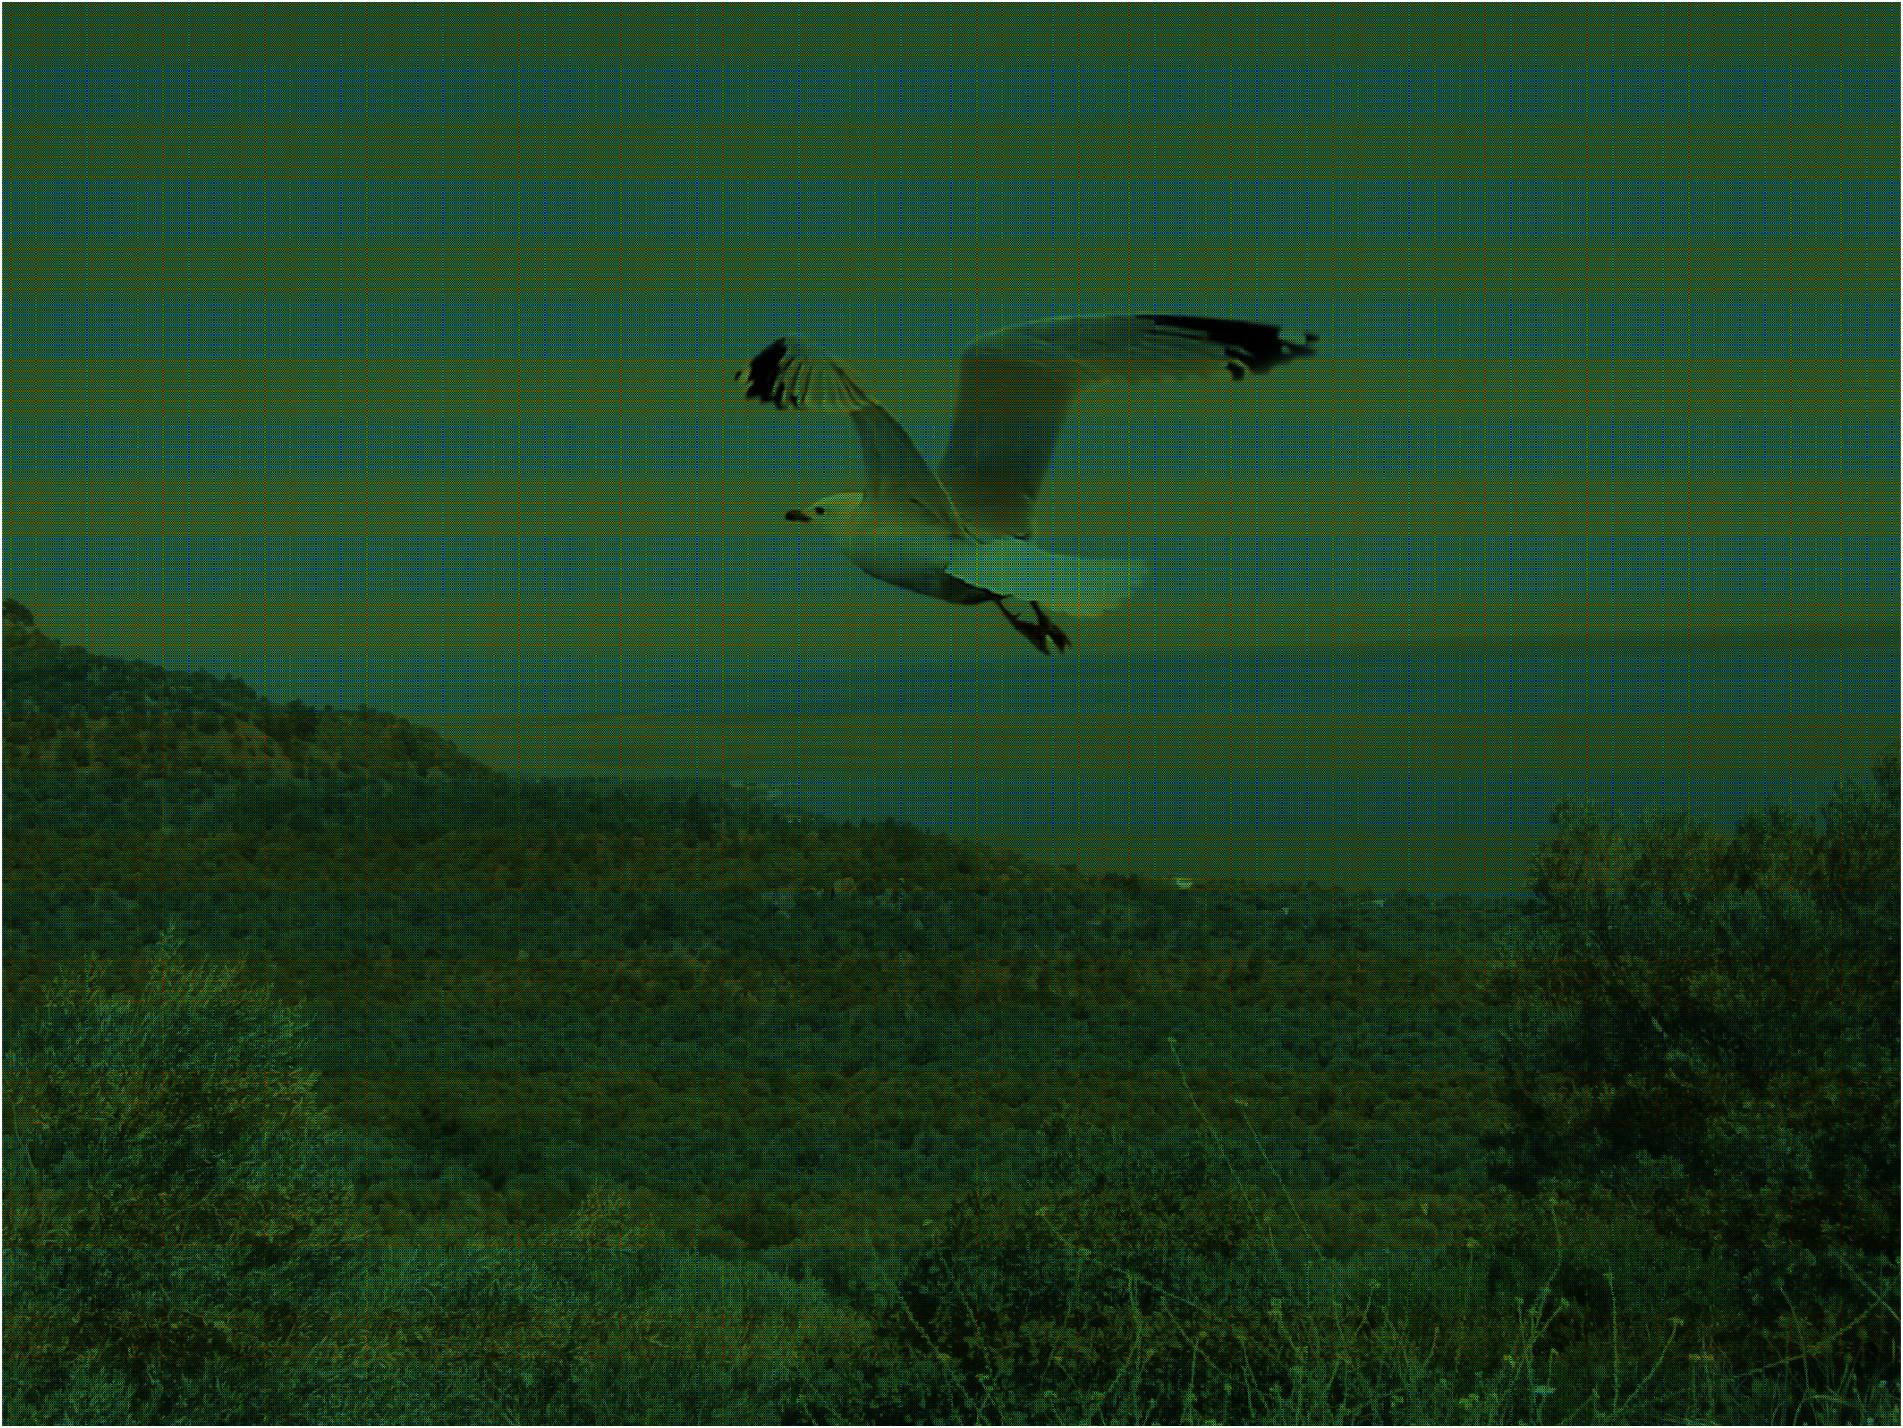
\includegraphics[trim=0 0 0 0,clip,width=\linewidth]{report/results/f1_steps_2.jpg}
        \caption{Re-sampled image}
    \end{subfigure}
    \hspace*{\fill}
    \begin{subfigure}{0.23\textwidth}
        \centering
        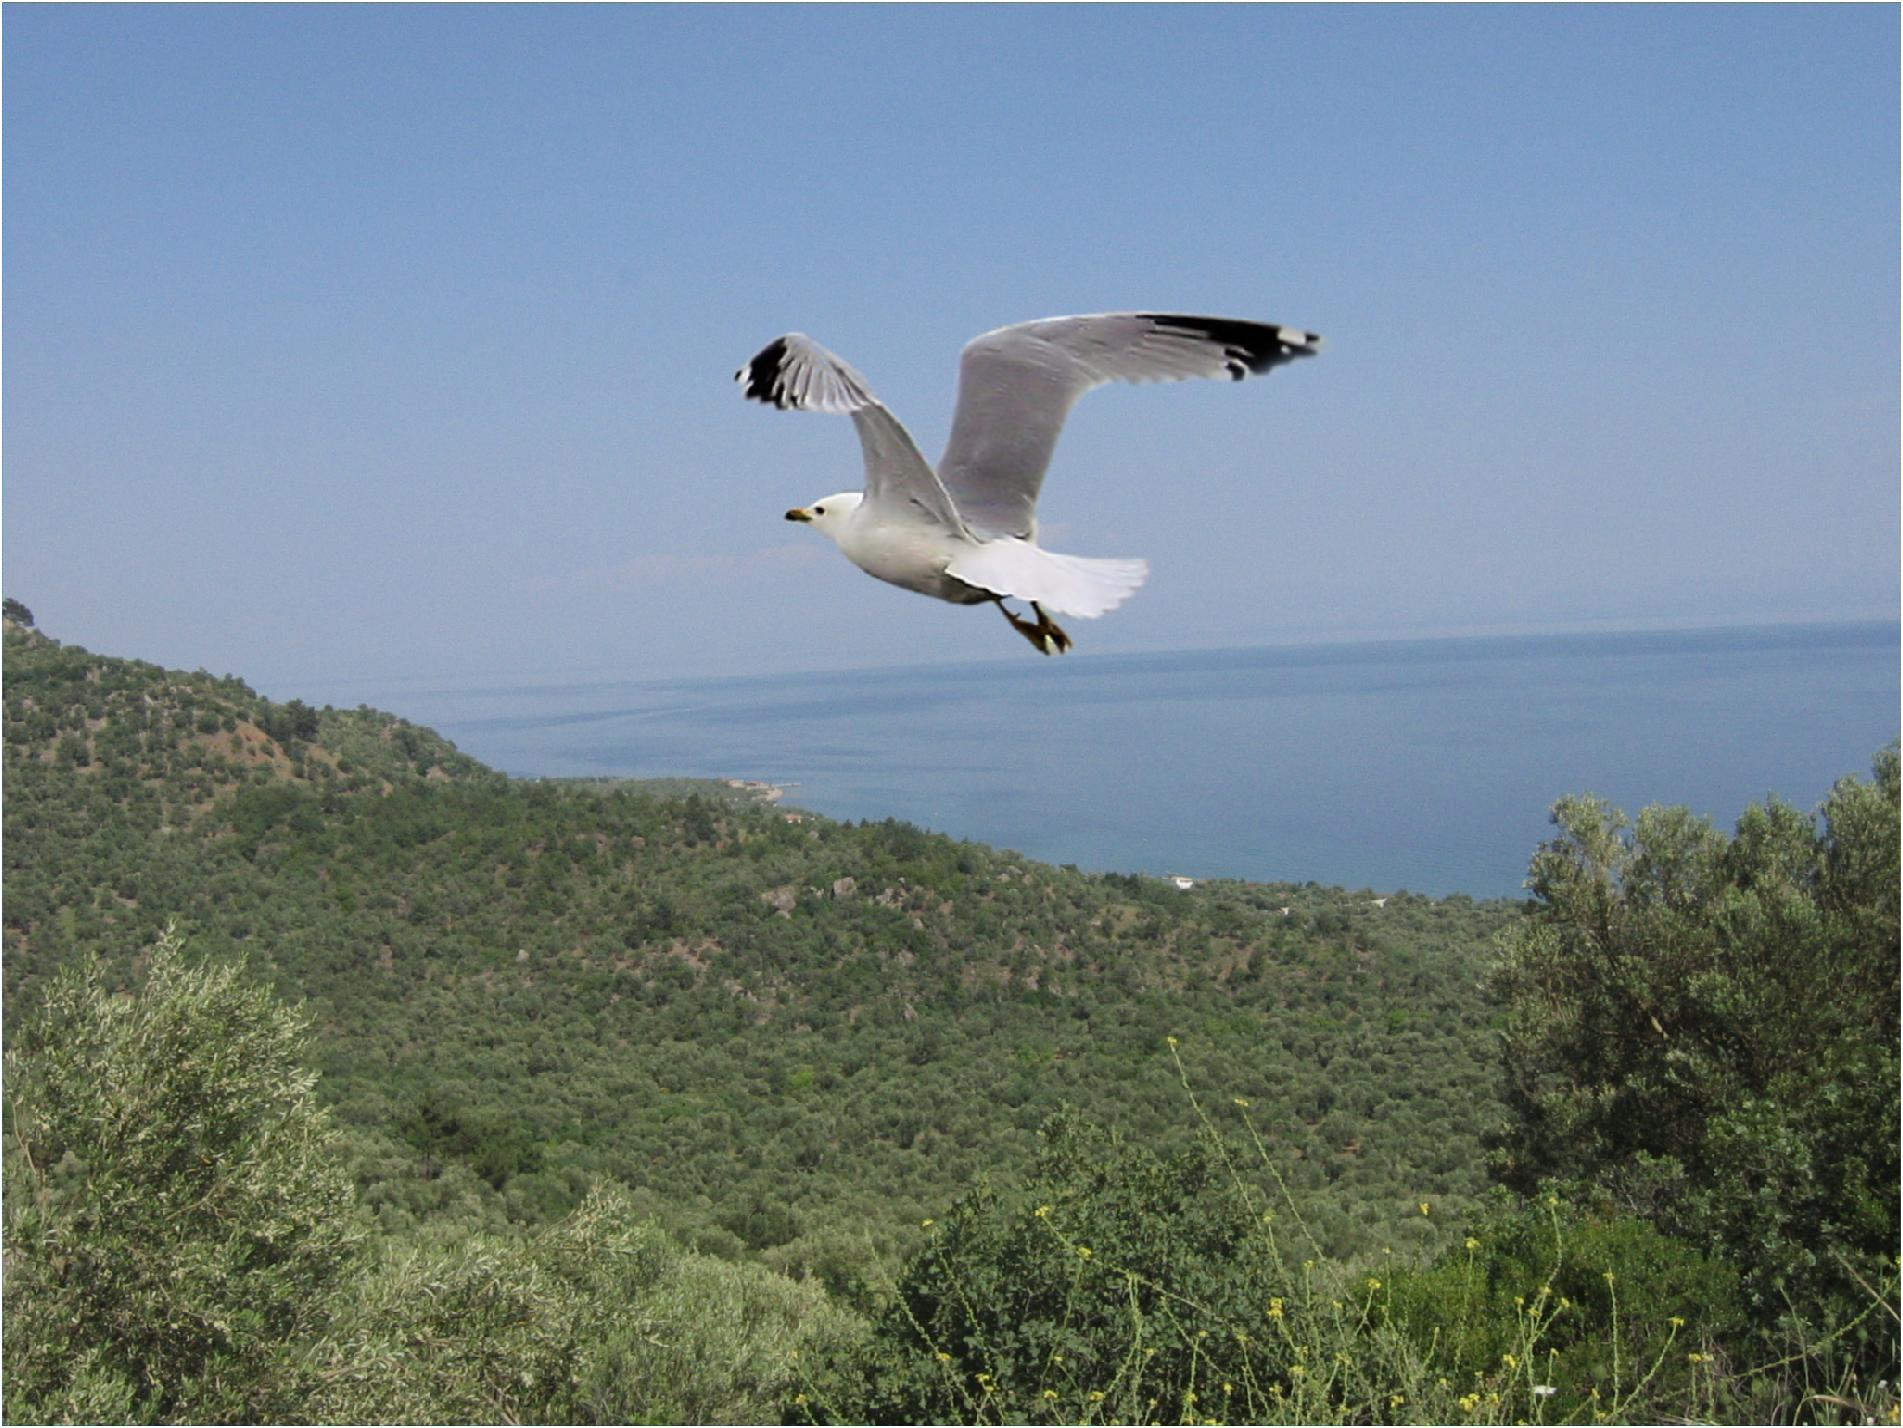
\includegraphics[trim=0 0 0 0,clip,width=\linewidth]{report/results/f1_steps_3.jpg}
        \caption{Re-interpolated image}
    \end{subfigure}
    
    \caption{F1 steps}
    \label{img_f1_steps}
\end{figure}

\subsection{Feature 2: CFA based noise analysis}

\section{Experiments}

\section{Conclusions}
TODO
shortcomings and problems

\bibliographystyle{abbrv}
\bibliography{main}

\end{document}
